% !TeX spellcheck = da_DK
\section{Gangfunktion}
Efterhånden som ALS-patienter mister muskelkraft, vil bevægeligheden i deres led nedsættes. Af denne grund opstår der kontrakturer i led, og muskelstramninger i de omkringliggende muskler.

Ved gang anvendes knæ-, hofte- og ankelleddet, hvilket fremgår af \autoref{fig:knaet}, hvis disse led ikke akviteres, opstår der muskelstramninger i benene \citep{instforms2008}.

\begin{figure} [H]
\centering
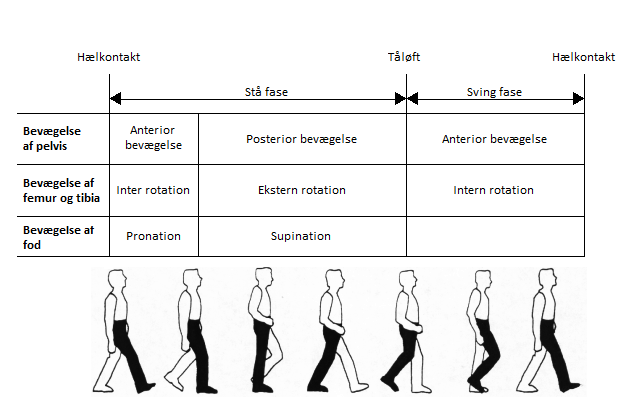
\includegraphics[width=0.9\textwidth]{figures/knaet}
\caption{Viser bevægelse af pelvis, femur og tibia samt foden ved forskellige faser under gang \citep{orthopedics2016}.}
\label{fig:knaet}
\end{figure} 

\noindent
Knæleddet vælges som udgangspunkt for et muligt body augmentation-system i form af et exoskelet, da knæleddet er et hængselled og derfor har et begrænset antal frihedsgrader. Knæleddet har én frihedsgrad, modsat andre mere komplekse led, hvilket gør, at leddet kun kan bevæge sig i én akse \citep{martini2012}. 
Det antages derfor, at knæleddet er et af de led, som er simplest at opbygge et system omkring. 
Hvis der kan laves et exoskelet omkring knæleddet, vil det kunne antages, at samme princip kan muliggøres ved henholdsvis hofte- og ankelleddet, hvorved gangfunktionen kan opretholdes.

\subsection{Knæets opbygning}
Knæet består af tre separate ledforbindelser. To, der er forbundet mellem femur og tibia, samt en mellem patella og femur, hvilket fremgår af \autoref{fig:knae_anatomi}. 

\begin{figure}[H]
\centering
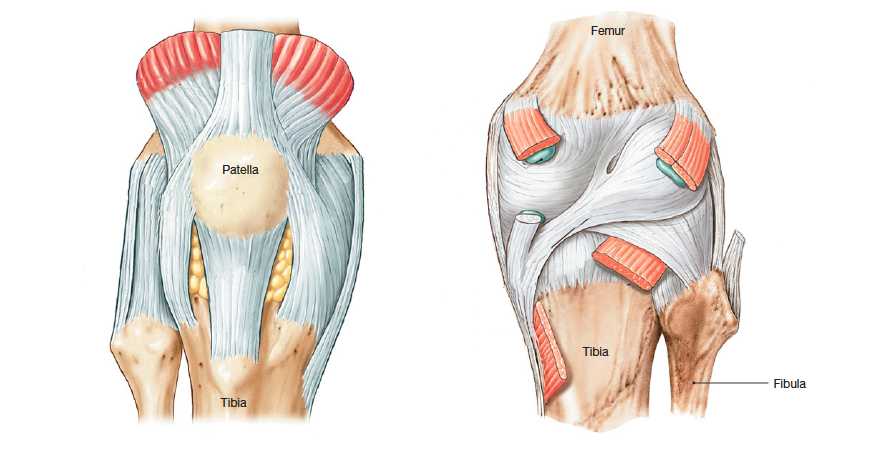
\includegraphics[width=0.8\textwidth]{figures/knae_anatomi}
\caption{Knæets anatomiske opbygning samt knæets forreste og bagerste korsbånd. \citep{aaos2014}.}
\label{fig:knae_anatomi}
\end{figure} 

\noindent
Ud over de tre separate ledforbindelser stabiliseres knæet af syv ledbånd. Ét af de syv ledbånd er patellarsenen, som er ansvarlig under extension af knæet. Derudover strækker to ledbånd sig mellem femur, tibia og fibia, hvilket er med til at styrke knæleddets overflade posteriort. 
Inde i ledkapslen befinder det forreste korsbånd, Anterior Cruciate Ligament (ACL), og det bagerste korsbånd, Posteior cruciate ligament (PCL), sig. Disse har til opgave at fastgøre indre knoglefremspring af tibia til knoglefremspringet på femur. 
Korsbåndene har til opgave at begrænse anteriore og posteriore bevægelser af femur og er med til at opretholde retningen af knoglefremspringene. 
Det tibiale kollaterale ligament forstærker den mediale flade af knæleddet, og det fibulære kollaterale ligament forstærker sidefladen. Disse ligamenter anvendes kun ved fuld ekstension af knæleddet \citep{martini2012}.

\subsection{Knæets funktion}
Ved gang aktiveres quadricepsmusklerne, der sidder anteriort på femur, og hasemusklerne, der sidder poseriort på femur. Nogle af disse muskler fremgår af \autoref{fig:laarmuskler}. Quadricepsmusklerne består af rectus femoris, vastus intermedius, vastus medialis og vastus lateralis. 
Hasemusklerne består af biceps femoris, semitendinosus og semimembranosus. 
Ved bevægelse foretager quadriceps- eller hasemusklerne ekstension eller fleksion, hvorved de fungerer som hinandens agonister eller antagonister under bevægelse \citep{martini2012}. 

\begin{figure} [H]
\centering
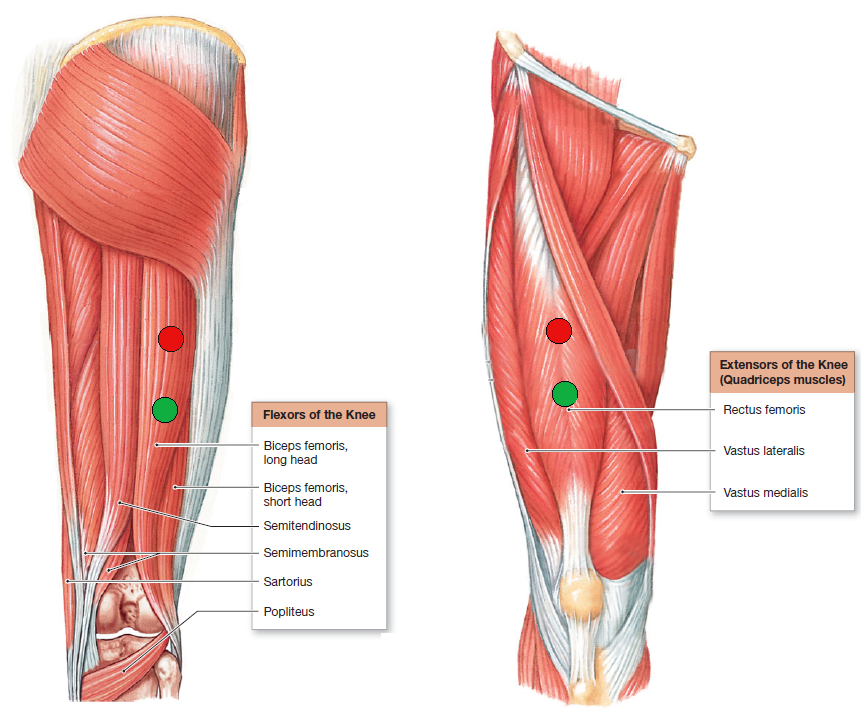
\includegraphics[width=0.9\textwidth]{figures/laarmuskler}
\caption{Viser rectus femoris, vastus lateris, biceps femoris, semimembranosus og patella  \citep{martini2012}.}
\label{fig:knaet}
\end{figure} 


Som tidligere nævnt anvendes hofte, knæ og ankler under gang. Udover disse led er kropsposituren og sving af leddene afgørende for gangfunktionen. Det fremgår af \autoref{fig:knaet}, hvordan de forskellige led udfører fleksion, ekstension og ændres fra ekstension til neutral bevægelse under gang \citep{martini2012}.

\subsubsection{Knæets funktion under en squat-øvelse} \label{sec:knaeled_squat}
% mere om, at det kun er lårets muskulatur, der benyttes under squat
Den dynamiske squat-øvelse er en udbredt træningsøvelse, som kræver styrke i flere muskelregioner. Squat aktiverer primært hofte-, lår- og rygmuskulaturen, som alle er primære muskler under gang, løb, spring og løft. Herudover anvendes squat som et redskab til rehabilitering af knæet, hvilket skyldes den måde, som knæet belastes under squat \citep{escamilla2001}. 

Knæets funktion for bøjningen af benet kan dermed ses ved udførelse af en squat-øvelse. En squat-øvelse udføres ved at stå i en oprejst position med knæ og hofte fuldt udstrakt. Herefter udføres en squat-øvelse i en kontinuerlig bevægelse, indtil den ønskede dybde nåes, hvorefter der udføres en kontinuerlig bevægelse tilbage til oprejst position \citep{escamilla2001}. En illustation af en squat-øvelse ses på \autoref{fig:squat}.

\begin{figure}[H]
\centering
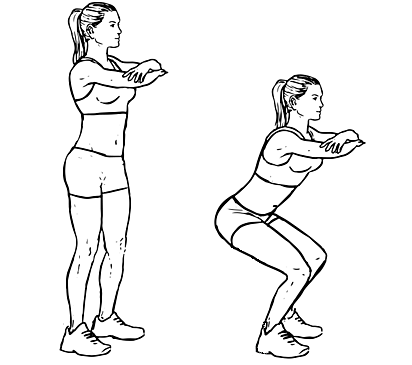
\includegraphics[width=0.5\textwidth]{figures/squat.png}
\caption{En illustration af udførelse af en halv squat-øvelse. Til venstre ses udgangspositionen, og til højre ses en halv squat-øvelse \citep{squat2015}.}
\label{fig:squat}
\end{figure}

\noindent 
Squat-øvelser kan udføres med varierende fleksion af knæet. De mest anvendte varianter af øvelsen er halv eller fuld squat. En halv squat-øvelse udføres indtil lårene er parallelle med jorden, hvilket svarer til en fleksion af knæet fra omkring $90-180^{\circ}$. En fuld squat-øvelse udføres indtil det posteriore del af låret og læggen kommer i kontakt med hinanden. Den fulde squat-øvelse anbefales mere trænede personer, hvorfor den halve squat-øvelse typisk er foretrukket til genoptræning af knæet \citep{escamilla2001}.

Ved udførelse af en squat-øvelse aktiveres blandt andet musklen rectus femoris. Aktiviteten i rectus femoris, og de resterende quadricepsmuskler, er størst ved $90-100^{\circ}$ vinkel af knæleddet \citep{schoenfeld2010}. 
Fra udgangspositionen for squat-øvelsen, der illustreres på \autoref{fig:squat}, befinder personen i en oprejst posistion med en vinkel på $180^{\circ}$ over knæet. Ved udførelse af en squat-øvelse vil muskelaktiviteten i rectus femoris være progressivt stigende indtil en vinkel over knæet på $90-100^{\circ}$ opnås. Idet der returneres til udgangspositionen, vil muskelaktiviteten være progressivt faldende \citep{escamilla2001}. 

%Biceps femoris aktiveres ved en $45^{\circ}$ fleksion af knæleddet, mens rectus femoris aktiveres ved en $80-90^{\circ}$ fleksion, hvorefter aktiviteten i musklerne er konsistent \citep{schoenfeld2010}. 


%Under en squat-øvelse aktiveres vastus intermedius, vastus medialis samt vastus lateris mere, da disse muskler er én ledmuskel, end rectus femoris der er en to-ledsmuskel \fxnote{hvorfor aktiveres én-ledsmuskler mere end to-ledsmuskler - jeg kan ikke finde det med hasemusklerne i den kilde der står til afsnittet?}.
%der er forbundet mellem femur, tibia og patella. Knæet har fire ledbånd. To af disse er side-ligamenterne, der sidder omkring knæleddet. De resterende to er korsbåndene, der sidder på skrå inden i knæet.
%Knæet fire ledbånd sikrer stabilisering af knæet og sørger for at knoglerne bevæger sig rigtigt.  Det er knæleddet, der gør det muligt for kroppen at kunne udføre aktiviteter som at kunne gå, løbe, og eksempelvis squatte. Ved gang aktiveres både quadriceps musklerne (rectus femoris, vastus intermedius, vastus medialis, vastus lateralis) der sidder anteriort for låret samt hamstring musklerne (biceps femoris, semitendinosus, Semimembranosus), der sidder posteriort for låret og kontraherer med quadriceps musklerne. 

